\documentclass[11pt]{article}
\usepackage[margin=1in]{geometry}
\usepackage{graphicx}
\usepackage{float}
\usepackage{booktabs}
\usepackage{array}
\usepackage{longtable}
\usepackage{hyperref}
\usepackage{enumitem}
\usepackage{amsmath}
\usepackage{caption}

\title{ECE 445 Senior Design Laboratory \\ Design Document \\ \vspace{0.5em} Intelligent Net-Energy-Optimized Solar Tracker}
\author{
Team \#48 \\
Minghao Fang \\
Ziru Niu \\
Yifei Liu \\
Yikai Zhang \\
Advisor: \texttt{TODO}
}
\date{April 1, 2026}

\begin{document}
\maketitle
\tableofcontents
\newpage

\section{Introduction}

\subsection{Problem Statement}
Small photovoltaic platforms lose energy when a fixed panel does not face the dominant light direction. A simple motorized tracker does not automatically solve that problem, because each movement consumes electrical energy and introduces mechanical wear. Under weak sunlight, cloud cover, or fast-changing illumination, a tracker can easily spend more energy turning the panel than it gains from the improved panel angle. Most low-cost student solar trackers are designed to maximize motion toward light, but not to determine whether that motion produces positive net energy gain.

This project addresses that gap with a dual-axis solar-tracking test platform that explicitly measures both generated panel power and motor-consumption power. The system uses a lower-level STM32 controller for sensing, actuation, and safety, and a Raspberry Pi for online inference and logging. The goal is not only to point the panel toward brighter light, but to decide when movement is worth the energy cost.

\subsection{Solution Overview and Visual Aid}
The project is organized around the top-level hardware chain in \texttt{TopLevel.txt}. A small solar panel is connected through an \texttt{INA219} monitor to a dummy load so the panel output can be measured without using the panel to power the controller. A second \texttt{INA219} measures the motor-power branch. A \texttt{BH1750 + I2C mux + 16-sensor} light ring samples directional light around the panel. A custom STM32-centered control board reads the sensors, refreshes an OLED, executes homing and motion commands, and drives two \texttt{A4988} stepper-driver stages connected to two \texttt{NEMA17} motors for yaw and pitch motion. A Raspberry Pi exchanges state and target-angle commands with the STM32 over UART and serves as the online inference and logging node. Offline model training is performed on a PC or cloud host and the trained model is later exported to \texttt{ONNX} for Raspberry Pi deployment.

This architecture matches the project objective especially well because it makes net-energy accounting measurable. The panel test path, motor branch, light ring, and control path are all visible and instrumented. The system can therefore explain why it moved, why it stayed still, and whether the resulting action increased or decreased net energy gain.

\begin{figure}[H]
\centering
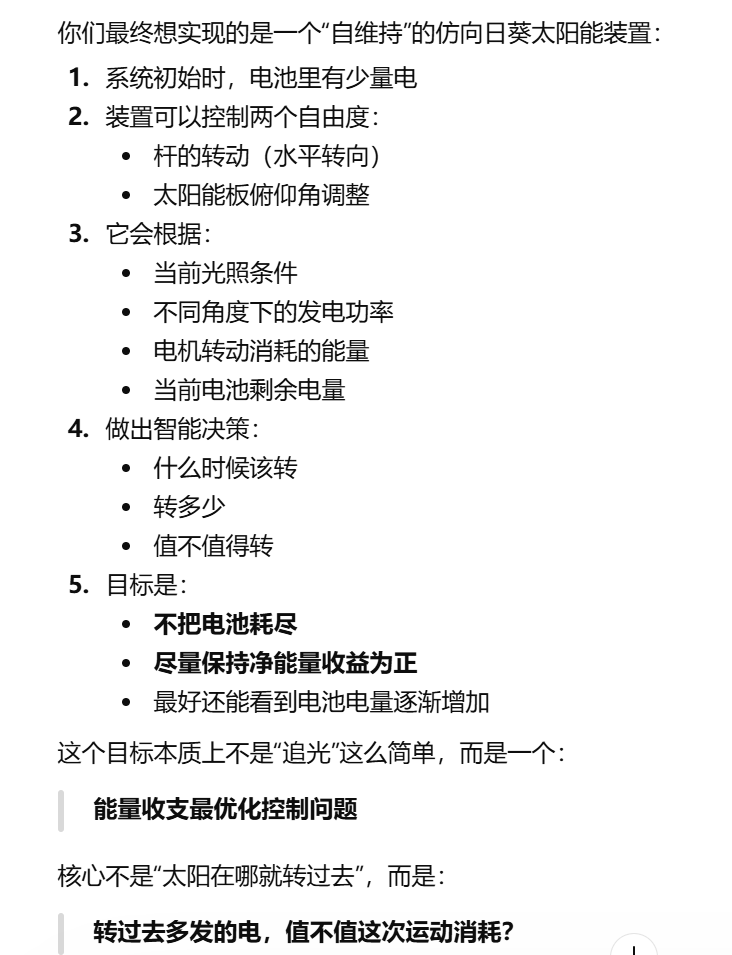
\includegraphics[width=0.62\linewidth]{High-Level-Design.png}
\caption{High-level visual aid derived from the current top-level hardware design. The figure shows the dual-axis tracker context, the panel measurement path, the STM32 lower-level controller, the Raspberry Pi inference node, the I2C sensing network, and the split 12 V and 5 V power architecture.}
\label{fig:visual-aid}
\end{figure}

\subsection{High-Level Requirements List}
The final system shall satisfy the following high-level requirements:

\begin{enumerate}[label=(\arabic*)]
\item \textbf{Autonomous startup:} After one button press, the system shall complete self-check and homing, then enter autonomous tracking mode without requiring a tethered computer.
\item \textbf{Tracking and net-gain behavior:} Under stable lighting, the platform shall track the brightest direction with steady-state pointing error less than $5^\circ$. Under weak or rapidly changing light, it shall avoid unnecessary actuation and demonstrate non-negative net energy gain relative to a naive always-move baseline during the same test window.
\item \textbf{Telemetry and visibility:} The OLED and host log shall update at least twice per second and report operating mode, panel voltage, panel current, motor-branch current, and current yaw/pitch state.
\end{enumerate}

\section{Design}

\subsection{Block Diagram}
The complete system contains six functional blocks: sensing, embedded control, online inference, actuation, power, and local user interface. The STM32F407ZGT6 is the hardware hub. It reads the shared I2C sensor network, drives the two motor axes, enforces homing and fault behavior, and exchanges data with the Raspberry Pi over UART. The Raspberry Pi receives current light-ring readings and current yaw/pitch state, runs the deployed model, and returns the next target angles. The two-axis mechanical structure converts these target angles into panel motion through \texttt{A4988} stepper drivers and \texttt{NEMA17} motors. The power system keeps the motor and logic branches separate so motor transients do not collapse the logic rail.

\begin{figure}[H]
\centering
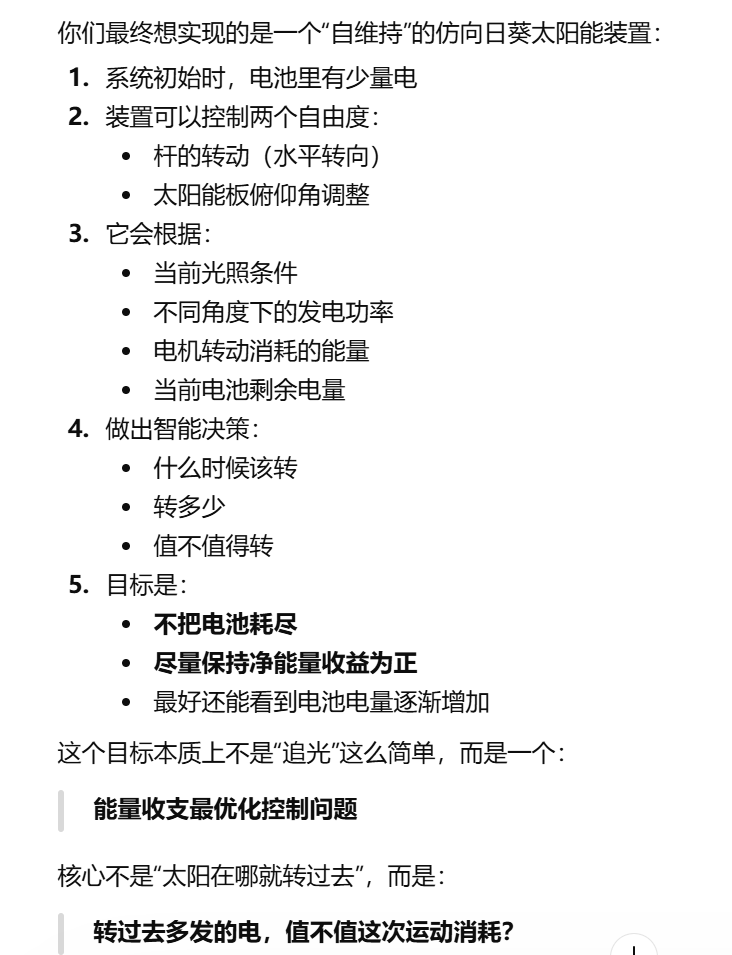
\includegraphics[width=0.74\linewidth]{High-Level-Design.png}
\caption{Whole-system block diagram based on the current top-level design. The solar panel feeds a measured dummy-load path, the STM32 reads the light ring and telemetry devices over I2C, the Raspberry Pi exchanges commands and state over UART, and the split 12 V and 5 V rails isolate motor power from logic power.}
\label{fig:block-diagram}
\end{figure}

\subsection{Mechanical and Actuation Subsystem}
The solar panel is mounted on a dual-axis frame with one yaw axis and one pitch axis. The current top-level design uses two \texttt{NEMA17} stepper motors and two \texttt{A4988} drivers. One axis handles east-west rotation and the other handles elevation adjustment. The STM32 outputs \texttt{STEP/DIR} style control signals, which keeps the electrical interface simple and makes angle commands easy to interpret.

This actuation approach is appropriate for the project because the main design question is not high-speed motion but measured, repeatable, energy-aware positioning. Open-loop step counting after homing is acceptable for a first implementation, provided startup calibration is reliable and the controller limits travel to safe ranges. In the current RL pipeline, the online current-angle state is defined as the previous target angle accepted by the STM32 after homing, not by an independent encoder.

\textbf{Subsystem requirements}
\begin{enumerate}[label=\arabic*.]
\item The yaw axis shall support at least $120^\circ$ of travel and the pitch axis shall support at least $60^\circ$ of travel.
\item Both axes shall home successfully on startup using limit switches or equivalent end-stop detection.
\item The motor-driver stage shall remain within configured current and thermal limits during repeated move, reverse, and hold-position tests.
\end{enumerate}

\textbf{Verification}
\begin{enumerate}[label=\arabic*.]
\item Measure total yaw and pitch travel using a protractor or counted steps referenced to a calibrated angle marker.
\item Perform ten consecutive startup cycles and verify that homing finishes successfully each time without losing the reference position.
\item Record driver temperature and motor-branch current during repeated motion tests and confirm that the chosen \texttt{A4988} settings remain within safe operating limits.
\end{enumerate}

\begin{figure}[H]
\centering
\fbox{\rule{0pt}{2.0in}\rule{0.86\linewidth}{0pt}}
\caption{Mechanical subsystem placeholder. Replace with a dual-axis assembly drawing showing the yaw and pitch frame, motor placement, panel mount, and homing-switch locations.}
\label{fig:mechanical}
\end{figure}

\subsection{Sensing Subsystem}
The sensing subsystem combines directional sensing and electrical measurement. A \texttt{BH1750 + mux + 16-sensor ring} samples incident light around the panel so the controller can estimate the dominant light direction. The STM32 polls the mux and reads one channel at a time over I2C. \texttt{INA219\_1} measures the solar-panel test path into a dummy load, and \texttt{INA219\_2} measures the external 12 V motor branch. This combination gives the project both the directional information needed to track light and the power data needed to reason about net gain.

The sensor set follows the exact intent of the top-level design. The project does not assume that the brightest direction is always the correct decision. Instead, it measures whether moving the panel improves generated power enough to justify the motor energy required to do so.

\textbf{Subsystem requirements}
\begin{enumerate}[label=\arabic*.]
\item The STM32 shall sample the light ring and both \texttt{INA219} channels at an effective rate of at least 10 Hz.
\item The panel measurement path shall resolve voltage and current changes accurately enough to distinguish useful changes in generated power during controlled tracking experiments.
\item Sensor processing shall include filtering or decision deadband so transient shadows and measurement noise do not cause rapid oscillation.
\end{enumerate}

\textbf{Verification}
\begin{enumerate}[label=\arabic*.]
\item Sweep a directional light source around the panel and verify that the light-ring distribution shifts consistently with source position.
\item Compare both \texttt{INA219} channels against a bench multimeter at multiple operating points and confirm the error is small enough for design-level net-power comparison.
\item Inject noisy or rapidly changing light conditions and verify that the filtered light estimate and motion decision remain stable.
\end{enumerate}

\begin{figure}[H]
\centering
\fbox{\rule{0pt}{2.0in}\rule{0.86\linewidth}{0pt}}
\caption{Sensor subsystem placeholder. Replace with a diagram showing the BH1750 light ring through the mux, the panel-to-dummy-load path through \texttt{INA219\_1}, and the motor-branch path through \texttt{INA219\_2}.}
\label{fig:sensing}
\end{figure}

\subsection{Control and Communication Subsystem}
The control subsystem is centered on the STM32F407ZGT6. It handles sensor polling, OLED refresh, state-machine logic, homing, motor-command execution, and safety enforcement. The current board-level interface assignment is consistent with the hardware notes: \texttt{PB6} and \texttt{PB7} are used for I2C \texttt{SCL/SDA}; \texttt{PA8} and \texttt{PA9} are used for yaw and pitch \texttt{STEP}; and \texttt{PB0/PB1} and \texttt{PB10/PB11} provide the direction and enable-style signals for the two axes. The Raspberry Pi is connected over a simple UART header and acts as the formal online inference node.

At the RL boundary, the STM32 uploads only the online state needed for deployment: current light-ring readings and current yaw/pitch state, where current angle is defined as the previous accepted target angle after homing. The Raspberry Pi runs inference and returns the next target angles. Logged electrical telemetry remains available for reward design, offline analysis, and evaluation, but is not required by the online model input. This division keeps the live interface small and feasible while preserving richer data for later training.

\textbf{Subsystem requirements}
\begin{enumerate}[label=\arabic*.]
\item The shared I2C bus shall support the OLED, both \texttt{INA219} devices, and the mux controller without address conflict.
\item The STM32 shall enforce safe motor behavior even if the Raspberry Pi stalls, disconnects, or returns invalid commands.
\item The UART protocol shall support deterministic state upload and target-angle return with bounded timeout behavior.
\end{enumerate}

\textbf{Verification}
\begin{enumerate}[label=\arabic*.]
\item Scan the I2C bus and verify that the OLED and both \texttt{INA219} devices respond at their intended addresses while the mux remains selectable.
\item Disconnect or pause the Raspberry Pi during active operation and verify that the STM32 transitions to a safe stop or hold mode.
\item Timestamp sent and received UART frames and confirm that the STM32-to-Pi-to-STM32 loop remains within the chosen control-period budget.
\end{enumerate}

\begin{figure}[H]
\centering
\fbox{\rule{0pt}{2.0in}\rule{0.86\linewidth}{0pt}}
\caption{Control and communication placeholder. Replace with a signal-flow diagram showing I2C peripherals on the STM32 side, the UART link to Raspberry Pi, and the target-angle return path to the two \texttt{A4988} driver stages.}
\label{fig:control}
\end{figure}

\subsection{Power Subsystem}
The current top-level design uses two external supplies. A 12 V adapter powers the motor branch and both \texttt{A4988} drivers. A separate 5 V rail powers the Raspberry Pi and the STM32 logic branch. The solar panel is not used as the controller power source; instead it is treated as a measured source under test. Its output flows through \texttt{INA219\_1} into a dummy load so the system can measure generated electrical power independently of the control electronics. The external motor branch is monitored by \texttt{INA219\_2}. This arrangement makes the energy accounting much clearer during verification and avoids unstable bring-up caused by trying to self-power the logic from a small test panel.

The PCB should expose clear test points for \texttt{12V}, \texttt{5V}, \texttt{3V3}, \texttt{GND}, I2C, UART, and motor supply nodes. Strong-current and weak-signal regions should be laid out separately so motor noise does not corrupt the sensor bus.

\textbf{Subsystem requirements}
\begin{enumerate}[label=\arabic*.]
\item The logic supply shall remain within tolerance during worst-case motor startup and reversal events.
\item The panel path and motor path shall both provide telemetry sufficient for net-power calculation during experiments.
\item The 12 V motor branch and 5 V logic branch shall be partitioned and protected against reverse polarity, short circuit, and wiring faults.
\end{enumerate}

\textbf{Verification}
\begin{enumerate}[label=\arabic*.]
\item Monitor the 5 V rail during aggressive motion tests and verify that no brown-out or logic reset occurs.
\item Compare sensor-based power estimates against external instrument measurements under several light and load conditions.
\item Validate the staged bring-up sequence by checking each rail and interface at dedicated test points before full electromechanical integration.
\end{enumerate}

\begin{figure}[H]
\centering
\fbox{\rule{0pt}{2.0in}\rule{0.86\linewidth}{0pt}}
\caption{Power subsystem placeholder. Replace with a power-tree diagram showing the external 12 V motor branch, the external 5 V logic branch, the panel-to-dummy-load measurement path, and the two \texttt{INA219} sensing points.}
\label{fig:power}
\end{figure}

\subsection{User Interface and One-Button Operation}
The local user interface is intentionally simple. A single button initiates startup. A 0.96-inch I2C OLED displays operating mode, panel voltage and current, motor branch telemetry, and current yaw/pitch state. This allows the system to be demonstrated without a laptop connected to the board.

The intended startup sequence is:
\begin{enumerate}[label=\arabic*.]
\item Power-on and self-test
\item Home the yaw and pitch axes
\item Start sensor polling and telemetry refresh
\item Enter normal tracking or energy-saving hold mode
\end{enumerate}

This directly supports the project requirement that the final platform behave as an autonomous device after one button press.

\begin{figure}[H]
\centering
\fbox{\rule{0pt}{1.8in}\rule{0.75\linewidth}{0pt}}
\caption{OLED display placeholder. Replace with a screen mockup showing mode, panel power, motor power, yaw angle, pitch angle, and any fault or hold-state indicator.}
\label{fig:oled}
\end{figure}

\subsection{Tolerance Analysis}
One critical tolerance is panel pointing error. For a flat photovoltaic panel under approximately direct illumination, the captured power can be approximated by
\begin{equation}
P(\theta) = P_{\max}\cos(\theta)
\end{equation}
where $\theta$ is the misalignment between the panel normal and the dominant incoming light direction.

For a $5^\circ$ error,
\begin{equation}
\frac{P(5^\circ)}{P_{\max}} = \cos(5^\circ) \approx 0.996
\end{equation}
which implies only about a $0.4\%$ reduction in ideal captured power. For a $15^\circ$ error,
\begin{equation}
\cos(15^\circ) \approx 0.966
\end{equation}
which corresponds to about a $3.4\%$ reduction.

This result is important for the system-level control decision. Very small angle errors do not justify large motor actions because the recovered solar power may be tiny compared with the cost of moving and holding the panel. The controller should therefore apply a motion deadband and only command new target angles when the expected gain is large enough to overcome the measured motor cost. The exact deadband can be tuned experimentally using the two \texttt{INA219} channels and the dummy-load measurement setup.

\begin{figure}[H]
\centering
\fbox{\rule{0pt}{2.0in}\rule{0.82\linewidth}{0pt}}
\caption{Tolerance-analysis placeholder. Replace with a cosine-loss curve or geometry sketch showing how pointing error affects captured panel power and motivates a no-move deadband.}
\label{fig:tolerance}
\end{figure}

\section{Cost}

Table~\ref{tab:cost} summarizes the current estimated project cost based on the hardware system of record in \texttt{docs/hardware/}. The design remains below the 1500 RMB budget target and leaves reserve for PCB iteration and mechanical integration.

\begin{longtable}{p{0.43\linewidth} p{0.09\linewidth} p{0.14\linewidth} p{0.14\linewidth}}
\caption{Estimated hardware cost.\label{tab:cost}}\\
\toprule
Item & Qty & Unit (RMB) & Subtotal (RMB) \\
\midrule
STM32F407ZGT6 development board & 1 & 80 & 80 \\
NEMA17 stepper motor & 2 & 80 & 160 \\
A4988 stepper driver & 2 & 20 & 40 \\
INA219 sensor module & 2 & 18 & 36 \\
BH1750 light sensor & 16 & 8 & 128 \\
I2C mux module or IC & 1 & 20 & 20 \\
0.96 in I2C OLED & 1 & 20 & 20 \\
12 V 5 A adapter & 1 & 45 & 45 \\
5 V logic supply & 1 & 20 & 20 \\
Push button, connectors, test points & 1 set & 35 & 35 \\
Solar panel & 1 & 80 & 80 \\
Dummy-load parts & 1 lot & 25 & 25 \\
PCB fabrication and passive parts & 1 lot & 180 & 180 \\
Mechanical couplings and brackets & 1 lot & 150 & 150 \\
\midrule
Total &  &  & 1019 \\
\bottomrule
\end{longtable}

The current estimate leaves about 481 RMB of reserve under the 1500 RMB budget cap.

\section{Schedule}

Table~\ref{tab:schedule} gives a draft milestone schedule aligned with the current team scope split.

\begin{longtable}{p{0.12\linewidth} p{0.52\linewidth} p{0.24\linewidth}}
\caption{Draft schedule and ownership.\label{tab:schedule}}\\
\toprule
Week & Main task & Owner \\
\midrule
1 & Freeze requirements, interfaces, and top-level architecture & Whole team \\
2 & Finalize component selection and cost model & Ziru, Yifei, Minghao \\
3 & Define UART protocol and STM32 pin allocation & Minghao, Ziru \\
4 & Draft schematic and power partitioning plan & Minghao, Yifei \\
5 & Bring up STM32 sensor reads on I2C & Minghao \\
6 & Bring up A4988 motor control and homing logic & Minghao, Ziru \\
7 & Integrate Raspberry Pi UART communication and logging & Minghao \\
8 & Prototype inference pipeline and ONNX deployment & Minghao \\
9 & Build and align dual-axis mechanical frame & Yikai, Whole team \\
10 & Integrate electronics with frame and verify power rails & Whole team \\
11 & Run tracking, power, and net-gain experiments & Whole team \\
12 & Finish document, figures, and final demonstration prep & Whole team \\
\bottomrule
\end{longtable}

\section{Ethics and Safety}

\subsection{Ethics}
The project must present energy-saving claims honestly. It would be misleading to claim that a moving solar tracker always improves performance. The core purpose of this project is to test when motion helps and when motion hurts net energy gain. The team should therefore report both positive and negative cases, clearly distinguish measured net gain from theoretical geometric gain, and state that the present platform is an externally powered test system rather than a self-powered photovoltaic node.

The project should also communicate the RL interface honestly. The online inference path uses only light-ring readings and current yaw/pitch state, while richer electrical telemetry is reserved for logging, training, and evaluation. Hiding that distinction would overstate the capability of the deployed model. These choices align with the IEEE Code of Ethics, especially the responsibility to be honest and realistic in stating claims and to improve understanding of technology and its appropriate application.

\subsection{Safety}
The project involves rotating mechanical parts, bench power supplies, exposed wiring during bring-up, and a mixed-signal PCB carrying both motor and logic paths. Key safety measures include:
\begin{itemize}
\item homing switches and software travel limits to prevent over-rotation,
\item current-limited \texttt{A4988} configuration and protected motor wiring,
\item mechanically secure mounting of the panel and moving frame,
\item insulated and strain-relieved power wiring with a controlled common ground,
\item staged low-voltage bench testing before full electromechanical operation,
\item clear emergency-stop or power-disconnect procedure during motion tests.
\end{itemize}

During verification, the team should keep hands clear of pinch points, test on a stable bench fixture, and confirm that no rail is energized beyond its intended rating before connecting the Raspberry Pi, STM32, or sensors.

\section{References}

\begin{enumerate}
\item IEEE, ``IEEE Code of Ethics,'' [Online]. Available: \url{https://www.ieee.org/about/corporate/governance/p7-8.html}
\item STMicroelectronics, ``STM32F407xx advanced Arm-based 32-bit MCUs,'' datasheet.
\item Texas Instruments, ``INA219 zer\=o-drift, bidirectional current/power monitor with I\textsuperscript{2}C interface,'' datasheet.
\item Texas Instruments, ``DRV/A4988-compatible stepper motor driver module documentation,'' vendor datasheet or carrier documentation.
\item Rohm Semiconductor, ``BH1750FVI digital ambient light sensor IC,'' datasheet.
\item \texttt{TODO}: Add the final I2C mux part number, selected NEMA17 motor datasheet, OLED module reference, and the exact external 12 V and 5 V supply references used in the final build.
\end{enumerate}

\end{document}
